\chapter{L'illusione di essere razionali}

\begin{flushright}
	\textit{``L'uomo \`{e} un animale razionale che perde sempre le staffe quando gli viene chiesto di agire secondo i dettami della ragione.''}\\[6pt]
	\textsc{\index[main]{Wilde, Oscar}Oscar Wilde}
\end{flushright}

\bigskip

\section{Il teatro della decisione}

Siete al supermercato, fermi davanti allo scaffale dei cereali. Quarantasette tipi diversi vi fissano con i loro colori sgargianti, e avete tre secondi per decidere. Prendete quelli con il trenta per cento di zuccheri in meno, perch\'{e} sembrano pi\`{u} sani. Ma aspettate: in meno rispetto a cosa? Non importa. Avete gi\`{a} messo la scatola nel carrello e siete passati al reparto successivo.

Benvenuti nel teatro quotidiano della razionalit\`{a}, dove recitiamo la parte di decisori consapevoli mentre in realt\`{a} improvvisiamo seguendo un copione scritto milioni di anni fa. Abbiamo gi\`{a} visto come il cervello trasformi i numeri in narrazioni e le probabilit\`{a} in premonizioni. Ma c'\`{e} qualcosa di ancora pi\`{u} profondo in gioco: l'illusione stessa di essere creature razionali, capaci di valutare le opzioni e scegliere liberamente la migliore.

Questa convinzione, chiamiamola il \index[main]{mito del decisore razionale}\textbf{mito del decisore razionale}, \`{e} forse la pi\`{u} grande finzione che ci raccontiamo. Il problema non \`{e} soltanto che sbagliamo i calcoli probabilistici. \`{E} che l'intero processo decisionale \`{e} spesso una ricostruzione successiva, una storia che ci raccontiamo dopo che una parte di noi, sotto la soglia della coscienza, ha gi\`{a} scelto.

Il problema, del resto, \`{e} antichissimo. Gi\`{a} Baruch Spinoza, nel 1677, osservava che gli uomini si credono liberi solo perch\'{e} sono consapevoli delle proprie azioni ma ignorano le cause che le determinano.\footnote{Spinoza, B. (1677). \textit{Ethica, ordine geometrico demonstrata}. Pubblicazione postuma, Amsterdam.} Trecento anni dopo, le neuroscienze gli stanno dando ragione in modi che lui non avrebbe potuto immaginare. Negli anni Ottanta Benjamin Libet applic\`{o} degli elettrodi sulla testa di alcuni volontari e chiese loro di muovere il polso quando ne avessero avuto voglia, annotando il momento preciso in cui diventavano consapevoli della decisione. Scopr\`{i} qualcosa di sconcertante: il cervello cominciava a prepararsi al movimento circa mezzo secondo \textit{prima} che la persona si rendesse conto di volersi muovere.\footnote{Libet, B., Gleason, C. A., Wright, E. W., e Pearl, D. K. (1983). Time of conscious intention to act in relation to onset of cerebral activity. \textit{Brain}, 106(3).} In altre parole, quando pensiamo ``adesso muovo il polso'', il cervello ha gi\`{a} deciso da un pezzo. La sensazione di scelta sembra arrivare dopo, come un'eco.

Ma allora chi decide davvero? E se non siamo noi, chi tiene il volante mentre guidiamo la macchina della nostra vita?

\section{Il decisore invisibile e l'elefante che porta il cavaliere}

Per capire come funzioni davvero il processo decisionale dobbiamo abbandonare l'immagine del cervello come computer razionale e adottarne una pi\`{u} fedele: il cervello come \index[cognitive]{macchina predittiva}macchina predittiva, che cerca continuamente di anticipare il futuro basandosi sul passato. Non valutiamo opzioni: confrontiamo schemi. Non scegliamo: riconosciamo.

Pensate a un grande maestro di scacchi. Garry Kasparov non analizzava tutte le mosse possibili, perch\'{e} le partite immaginabili sono pi\`{u} numerose degli atomi dell'universo. Guardava la scacchiera e ``vedeva'' la mossa giusta, all'istante. Solo dopo, se glielo chiedevano, costruiva una spiegazione logica del perch\'{e} quella mossa fosse superiore.\footnote{Kasparov, G., e Greengard, M. (2007). \textit{How Life Imitates Chess}. Bloomsbury, New York.} I ricercatori hanno studiato il fenomeno seguendo letteralmente lo sguardo dei grandi maestri davanti a una posizione, e hanno fatto una scoperta sorprendente: mentre i principianti saltano freneticamente da un pezzo all'altro esplorando decine di possibilit\`{a}, i maestri fissano nei primi cinque secondi le zone critiche della scacchiera.\footnote{Charness, N., Reingold, E. M., Pomplun, M., e Stampe, D. M. (2001). The perceptual aspect of skilled performance in chess: Evidence from eye movements. \textit{Memory and Cognition}, 29(8).} Non stanno cercando la mossa migliore: l'hanno gi\`{a} trovata. Il resto del tempo serve solo a verificare che l'intuizione sia corretta.

\`{E} lo stesso meccanismo che opera quando un medico esperto diagnostica una malattia rara con un'occhiata, quando un sommelier identifica un vino dall'aroma, quando vostra madre capisce che state mentendo prima ancora che apriate bocca. Non \`{e} magia, \`{e} \index[cognitive]{riconoscimento di schemi}riconoscimento di schemi portato a un livello sublime. Il cervello ha visto cos\`{i} tante configurazioni simili da riconoscere all'istante quelle significative, esattamente come voi riconoscete il volto di un amico tra mille persone in una stazione affollata. E quando chiediamo a questi esperti come facciano, loro inventano. Non mentono di proposito, credono sinceramente alle spiegazioni che forniscono. Kasparov potrebbe dirvi di aver scelto quella mossa ``per controllare il centro e preparare un attacco sul lato di re'', eppure gli studi con gli scanner cerebrali mostrano che la decisione era gi\`{a} presa prima che la parte analitica del cervello si attivasse.\footnote{Wan, X., e altri (2011). The neural basis of intuitive best next-move generation in board game experts. \textit{Science}, 331(6015).}

Il fenomeno non riguarda solo gli scacchi. Gary Klein ha studiato i vigili del fuoco esperti, costretti a decidere in una frazione di secondo se un edificio stia per crollare. Non fanno analisi costi benefici, non compilano liste mentali: ``sentono'' il pericolo. Un comandante gli raccont\`{o} di aver ordinato l'evacuazione immediata di un palazzo all'apparenza stabile. Trenta secondi dopo, croll\`{o}. Quando Klein gli chiese come avesse fatto a saperlo, il comandante cominci\`{o} a elencare indizi razionali: il colore del fumo, il suono delle travi, il calore del pavimento. Ma la verit\`{a} \`{e} che aveva semplicemente avvertito che qualcosa non andava. Le spiegazioni razionali erano arrivate dopo.\footnote{Klein, G. (1998). \textit{Sources of Power: How People Make Decisions}. MIT Press, Cambridge.}

Lo stesso meccanismo governa ogni nostra decisione quotidiana. Il decisore invisibile, quella vasta rete neurale che elabora informazioni sotto la soglia della coscienza, ha gi\`{a} compiuto la scelta. La mente cosciente arriva dopo, come un addetto stampa che deve spiegare ai giornalisti una decisione gi\`{a} presa dal consiglio di amministrazione. Jonathan Haidt ha trovato per tutto questo una metafora memorabile: la mente razionale \`{e} come un piccolo cavaliere seduto sopra un enorme elefante emotivo.\footnote{Haidt, J. (2006). \textit{The Happiness Hypothesis}. Basic Books, New York.} Il cavaliere pu\`{o} suggerire la direzione, tirare le redini, perfino illudersi di comandare. Ma quando l'elefante vuole andare a sinistra, a sinistra si va. E il cavaliere, invece di ammettere la propria impotenza, costruisce spiegazioni elaborate sul perch\'{e} andare a sinistra fosse proprio ci\`{o} che desiderava.

\begin{figure}[htbp]
	\centering
	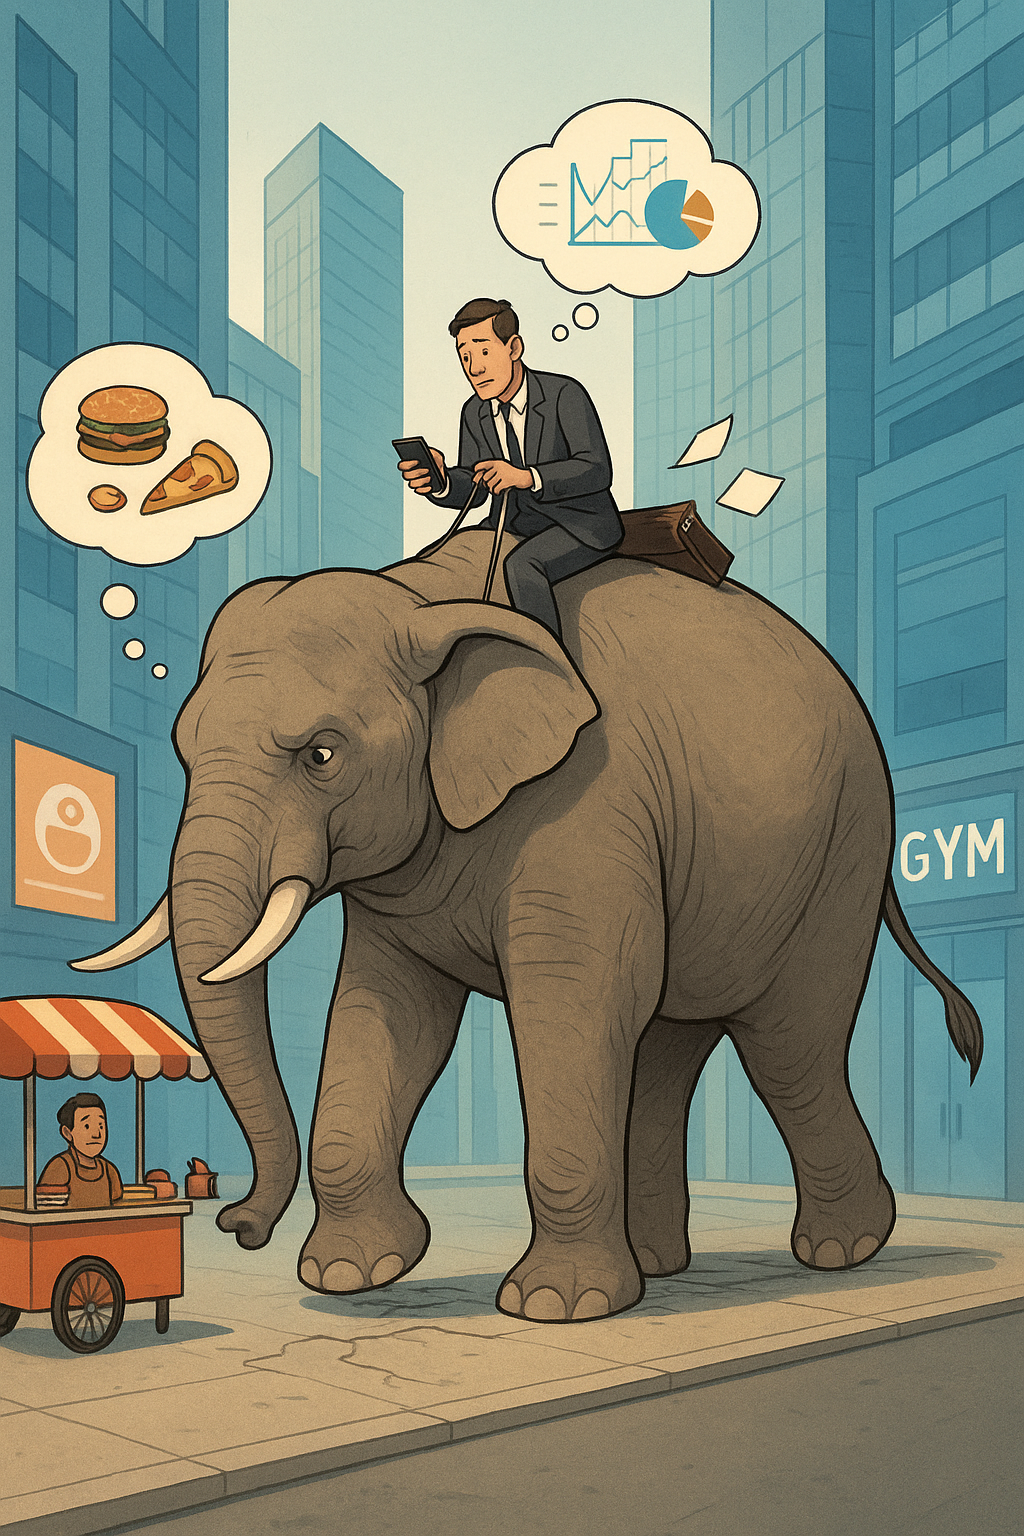
\includegraphics[width=1\textwidth]{images/elefante_mahout.png}
	\captionof{figure}{La metafora di Haidt per il rapporto tra mente razionale ed emotiva. Il piccolo cavaliere pu\`{o} suggerire la direzione, ma quando l'elefante decide non c'\`{e} discussione che tenga. L'immagine cattura l'illusione di controllo che sperimentiamo ogni giorno.}
	\label{fig:elephant_rider}
\end{figure}

Qui per\`{o} la storia si fa ancora pi\`{u} intrigante, perch\'{e} questo sistema funziona benissimo per un mondo che non esiste pi\`{u}. L'elefante emotivo \`{e} stato addestrato per milioni di anni a riconoscere schemi di sopravvivenza: pericolo o sicurezza, commestibile o velenoso, amico o nemico. Schemi binari, immediati, vitali. Ma quarantasette tipi di cereali? Il mutuo a tasso variabile? La pensione integrativa? Per problemi simili l'elefante non ha ricevuto alcun addestramento. Ed \`{e} qui che emerge uno dei paradossi pi\`{u} curiosi della condizione umana: pi\`{u} opzioni abbiamo, pi\`{u} infelici diventiamo. Barry Schwartz lo chiama il \index[cognitive]{paradosso della scelta}paradosso della scelta.\footnote{Schwartz, B. (2004). \textit{The Paradox of Choice: Why More Is Less}. Ecco, New York.} Quando le opzioni erano due o tre, l'elefante sceglieva in fretta e il cavaliere inventava una storia semplice. Con quarantasette scatole di cereali l'elefante si confonde, il cavaliere va in tilt, e usciamo dal supermercato con l'angoscia di aver sbagliato tutto.

\section{Lo specchio opaco: perch\'{e} vediamo solo i bias degli altri}

C'\`{e} per\`{o} un secondo livello di illusione, ancora pi\`{u} insidioso. Non solo ci illudiamo di essere razionali: ci illudiamo di essere \textit{pi\`{u}} razionali degli altri. Il cavaliere \`{e} un eccellente diagnostico dei problemi altrui, ma soffre di una profonda miopia quando deve guardare il proprio elefante.

Gli psicologi chiamano questo fenomeno \index[cognitive]{punto cieco dei bias}punto cieco dei bias.\footnote{Pronin, E., Lin, D. Y., e Ross, L. (2002). The bias blind spot: Perceptions of bias in self versus others. \textit{Personality and Social Psychology Bulletin}, 28(3).} In uno studio illuminante i ricercatori spiegarono ai partecipanti come funziona questo meccanismo, ossia la tendenza a vedere i pregiudizi negli altri ma non in se stessi. Poi chiesero: ``E tu, quanto pensi di esserne affetto?'' La risposta tipica suonava cos\`{i}: ``Io no, io sono abbastanza consapevole dei miei bias''. Esattamente ci\`{o} che il punto cieco prevedeva. \`{E} come avere un telescopio che funziona alla perfezione quando lo puntiamo verso gli altri, ma diventa opaco appena cerchiamo di guardare noi stessi. Vediamo con chiarezza che Marco \`{e} irragionevolmente attaccato alla sua squadra, che Giulia nega ostinatamente i segnali di un tradimento, che Paolo si giustifica dopo ogni errore di investimento. Ma noi siamo diversi. Le nostre scelte sono ponderate, i nostri giudizi obiettivi, e le nostre razionalizzazioni, beh, quelle sono ragioni legittime, non razionalizzazioni.

Questo punto cieco si amplifica, paradossalmente, proprio dove la nostra competenza \`{e} minore. David Dunning e Justin Kruger hanno scoperto un fatto sconcertante: le persone meno competenti in un ambito sono spesso le pi\`{u} sicure delle proprie capacit\`{a}.\footnote{Kruger, J., e Dunning, D. (1999). Unskilled and unaware of it: How difficulties in recognizing one's own incompetence lead to inflated self-assessments. \textit{Journal of Personality and Social Psychology}, 77(6).} Non per arroganza, ma per un motivo pi\`{u} sottile: \`{e} proprio la mancanza di competenza a impedirci di riconoscere i nostri errori. Per capire di aver suonato male una sonata di Chopin dovete sapere come suona eseguita bene; per riconoscere un algoritmo scritto male dovete conoscere i principi della buona programmazione. L'\index[cognitive]{effetto Dunning-Kruger}effetto Dunning-Kruger non \`{e} dunque semplice presunzione: \`{e} un'incapacit\`{a} metacognitiva. Non sappiamo di non sapere, perch\'{e} sapere di non sapere richiederebbe esattamente le competenze che ci mancano. \`{E} come guidare con gli occhi bendati, convinti di vederci benissimo perch\'{e} non ci accorgiamo di avere la benda.

C'\`{e} infine un terzo strato in questa matrioska dell'autoinganno: la \index[cognitive]{superiorit\`{a} illusoria}superiorit\`{a} illusoria. Interrogati sul punto, il novantatr\'{e} per cento degli automobilisti americani si giudica ``sopra la media'' nella guida.\footnote{Svenson, O. (1981). Are we all less risky and more skillful than our fellow drivers? \textit{Acta Psychologica}, 47(2).} La maggioranza dei docenti universitari ritiene di insegnare meglio dei colleghi, e quasi nove studenti di management su dieci si considerano pi\`{u} capaci della media. Matematicamente impossibile, psicologicamente inevitabile. Non \`{e} narcisismo, \`{e} architettura mentale: per restare funzionali e motivati abbiamo bisogno di crederci almeno un po' speciali, un po' migliori, un po' pi\`{u} razionali degli altri. Un elefante depresso non sopravvive a lungo nella savana. Ma questa illusione ha un prezzo. Se siamo convinti di essere pi\`{u} lucidi degli altri, se pensiamo di vedere i nostri bias mentre loro restano ciechi ai propri, come potremo mai imparare davvero? Come correggeremo errori che, ai nostri occhi, sono sempre errori altrui?

\section{L'architetto della coerenza e il sistema immunitario dell'ego}

Il cervello ha per\`{o} un asso nella manica, un meccanismo cos\`{i} raffinato da riuscire a nascondere tutte queste contraddizioni: il \index[cognitive]{sistema di coerenza narrativa}sistema di coerenza narrativa. \`{E} come avere un romanziere interno che lavora ventiquattr'ore al giorno per riscrivere di continuo la nostra storia in modo che torni. L'architetto della coerenza \`{e} un genio dell'improvvisazione: prende decisioni contraddittorie, comportamenti incoerenti, cambi di opinione repentini, e li intreccia in una narrazione dove siamo sempre stati coerenti, sempre razionali, sempre noi stessi. \`{E} grazie a lui che possiamo dire con assoluta convinzione ``lo sapevo che sarebbe andata cos\`{i}'' dopo ogni evento, avendo del tutto rimosso le nostre previsioni opposte.

Carol Tavris ed Elliot Aronson hanno chiamato questo meccanismo la piramide dell'autogiustificazione.\footnote{Tavris, C., e Aronson, E. (2007). \textit{Mistakes Were Made (But Not by Me)}. Harcourt, Orlando.} Ogni piccola giustificazione ci porta un gradino pi\`{u} in alto, finch\'{e} ci ritroviamo in cima a una piramide di razionalizzazioni, persuasi di esserci sempre stati. Il fumatore non ammette la dipendenza: ``Mi rilassa, e lo stress fa peggio del fumo''. Chi ha comprato un'auto troppo cara non riconosce l'errore: ``\`{E} un investimento nella sicurezza della famiglia''. Chi resta in una relazione infelice riscrive la trama: ``L'amore vero richiede sacrificio''. Non sono scuse calcolate, sono convinzioni sincere, costruite in tempo reale, mattone dopo mattone, per un'unica ragione: mantenere intatta l'immagine che abbiamo di noi stessi.

Ma perch\'{e} il cervello \`{e} cos\`{i} ossessionato dalla coerenza, al punto da falsificare la realt\`{a}? La risposta \`{e} insieme semplice e profonda: perch\'{e} la contraddizione fa male, alla lettera. Quando crediamo una cosa e ne facciamo un'altra, quando i valori che dichiariamo contraddicono le nostre azioni, quando la realt\`{a} smentisce le nostre previsioni, sperimentiamo quella che gli psicologi chiamano \index[cognitive]{dissonanza cognitiva}dissonanza cognitiva. Non \`{e} un concetto astratto: \`{e} un dolore psicologico reale, visibile nelle scansioni cerebrali, accompagnato da uno stress fisiologico misurabile.\footnote{van Veen, V., Krug, M. K., Schooler, J. W., e Carter, C. S. (2009). Neural activity predicts attitude change in cognitive dissonance. \textit{Nature Neuroscience}, 12(11).}

Anche questa, per quanto possa sembrare una scoperta del Novecento, era gi\`{a} stata vista molto tempo fa. Quando Leon Festinger formul\`{o} la teoria della dissonanza nel 1957, non faceva che dare un nome sperimentale a ci\`{o} che Platone aveva descritto nella \textit{Repubblica} come l'anima in guerra con se stessa, lacerata tra parti che vogliono cose opposte.\footnote{Platone. \textit{La Repubblica}, libro IV. Numerose edizioni.} Il fumatore di oggi, che conosce alla perfezione i rischi e tuttavia accende l'ennesima sigaretta, \`{e} l'erede diretto di quell'antica figura del dialogo platonico: l'uomo che sa benissimo cosa sarebbe bene e fa puntualmente il contrario. \`{E} il problema che i filosofi greci chiamavano \index[main]{akrasia}\textit{akrasia}, la debolezza della volont\`{a}, e che attraversa intatto venticinque secoli per riaffacciarsi nei laboratori di neuroimmagine.

Il cervello, di fronte a questo dolore, attiva immediatamente una risposta immunitaria. Possiamo immaginare questo meccanismo come un \index[cognitive]{sistema immunitario dell'ego}sistema immunitario dell'ego: una rete di difese psicologiche automatiche che si mobilitano per proteggere l'autostima dall'assalto della realt\`{a}. L'anticorpo principale si chiama \index[cognitive]{ragionamento motivato}ragionamento motivato.\footnote{Kunda, Z. (1990). The case for motivated reasoning. \textit{Psychological Bulletin}, 108(3).} Noi crediamo che la ragione funzioni in un certo modo: osserviamo i fatti, valutiamo le prove, arriviamo a una conclusione. Nella realt\`{a} il processo \`{e} spesso rovesciato: arriviamo a una conclusione emotiva istantanea, e solo dopo la ragione si mette al lavoro per trovare argomenti che la sostengano. L'architetto della coerenza non \`{e} uno storico obiettivo, \`{e} un avvocato difensore il cui unico cliente siamo noi stessi. Il suo compito non \`{e} trovare la verit\`{a}, ma vincere la causa. Sempre.

Cos\`{i} ogni piccolo atto di autogiustificazione si trasforma, da semplice errore cognitivo, in medicina necessaria. Ogni volta che troviamo una scusa per un fallimento, che riscriviamo il passato per sembrare pi\`{u} saggi, che razionalizziamo una decisione sbagliata, prendiamo una dose di antibiotico cognitivo: il dolore della dissonanza si attenua, l'infezione viene contenuta, l'immagine di s\'{e} resta intatta. Il fenomeno diventa ancora pi\`{u} affascinante quando osserviamo come cambiamo opinione: non lo facciamo mai davvero. L'architetto riscrive il passato in modo che abbiamo sempre pensato ci\`{o} che pensiamo ora. ``Avevo sempre avuto dei dubbi su quella persona'', diciamo dopo che si \`{e} rivelata inaffidabile, dimenticando la fiducia iniziale. ``Sapevo che era l'investimento giusto'', proclamiamo dopo che le azioni sono salite, cancellando i mesi di incertezza. Gli psicologi lo chiamano \index[cognitive]{distorsione retrospettiva}distorsione retrospettiva, ma definirla soltanto distorsione \`{e} riduttivo: \`{e} il meccanismo con cui manteniamo un senso coerente di identit\`{a} in un mondo caotico.\footnote{Fischhoff, B. (1975). Hindsight is not equal to foresight: The effect of outcome knowledge on judgment under uncertainty. \textit{Journal of Experimental Psychology: Human Perception and Performance}, 1(3).}

Qui per\`{o} il discorso sfiora una soglia filosofica che vale la pena attraversare. Per secoli si \`{e} pensato che bastasse conoscere il bene per compierlo. Immanuel Kant, nel cuore dell'Illuminismo, costru\`{i} un'intera etica su questa fiducia nella ragione pura: l'imperativo categorico ci impone di agire sempre secondo una massima che potremmo desiderare valesse come legge universale, indipendentemente dalle nostre inclinazioni.\footnote{Kant, I. (1788). \textit{Kritik der praktischen Vernunft}. Riga.} Era un progetto magnifico, in cui la volont\`{a} razionale doveva poter zittire l'elefante emotivo con la sola forza del dovere. Eppure i bias cognitivi sono, in un certo senso, la smentita sperimentale di quel sogno: dimostrano che la conoscenza del dovere, da sola, non basta quasi mai a determinare il comportamento. Kant aveva ragione su come dovremmo agire; aveva torto, forse, sulla nostra reale capacit\`{a} di farlo. E tra il suo ottimismo e la nostra natura contraddittoria si apre proprio lo spazio in cui vive la dissonanza.

\section{La mala fede: quando l'autoinganno diventa una scelta}

C'\`{e} un'obiezione che a questo punto qualcuno potrebbe sollevare. Se tutto questo lavoro di razionalizzazione avviene sotto la soglia della coscienza, se l'architetto interno opera a nostra insaputa, allora non siamo davvero responsabili di nulla. Saremmo semplici spettatori di un teatro recitato da altri dentro di noi.

Un filosofo del Novecento ha rifiutato con forza questa scappatoia. Jean-Paul Sartre, nel suo \textit{L'essere e il nulla}, descrisse un fenomeno che chiam\`{o} \index[main]{mala fede}\textit{mala fede}: l'autoinganno attivo con cui fuggiamo dalla nostra stessa libert\`{a}.\footnote{Sartre, J. P. (1943). \textit{L'\^{e}tre et le n\'{e}ant}. Gallimard, Parigi.} Per Sartre fingere di non sapere ci\`{o} che in fondo sappiamo non \`{e} un incidente involontario, ma una forma sottile di scelta: scegliamo di non guardare, perch\'{e} guardare ci costringerebbe ad agire. Il cameriere che recita troppo perfettamente la parte del cameriere, l'innamorata che finge di non capire le intenzioni evidenti del corteggiatore, sono per lui figure di questa fuga. La mala fede \`{e} il velo che cala su una verit\`{a} scomoda, calato per\`{o} dalla nostra stessa mano.

\`{E} difficile non riconoscere, in questa intuizione, una versione filosofica esatta del ragionamento motivato. Ci\`{o} che la neuroscienza descrive come un automatismo del Sistema 1, Sartre lo legge come un atto, sia pure mascherato. E forse la verit\`{a} sta in mezzo: il meccanismo \`{e} automatico, ma resta sempre un margine, sottile e scomodo, in cui possiamo decidere se assecondarlo o interromperlo. Il fumatore che si racconta che lo stress fa peggio del fumo sta facendo qualcosa di pi\`{u} che subire un bias: in qualche angolo di s\'{e}, sta scegliendo di non vedere. \`{E} questa zona grigia, tra l'automatismo e la scelta, il vero campo di battaglia della libert\`{a} umana.

Ed \`{e} qui che si chiude un cerchio lungo venticinque secoli. La domanda che Sartre poneva nel 1943, quella che Kant aveva affrontato nel Settecento e Platone ancora prima, era stata formulata nei termini pi\`{u} netti da Aristotele nel settimo libro dell'\textit{Etica Nicomachea}.\footnote{Aristotele. \textit{Etica Nicomachea}, libro VII. Numerose edizioni.} Il filosofo si chiedeva come fosse possibile l'akrasia: come pu\`{o} un uomo sapere ci\`{o} che \`{e} bene e fare deliberatamente il contrario? Per Aristotele era uno dei paradossi fondamentali dell'etica, perch\'{e} sembrava contraddire l'idea stessa che la conoscenza guidi l'azione. La sua risposta, sorprendentemente moderna, fu che nel momento della passione la conoscenza si oscura, resta presente solo a parole, come un attore che recita un copione senza capirne il senso. Oggi diremmo che il sapere razionale del cavaliere viene messo offline dall'elefante emotivo. Aristotele non disponeva di scanner cerebrali, ma aveva gi\`{a} intuito la cosa essenziale: l'intelletto, da solo, non basta a governare il comportamento. La conoscenza \`{e} necessaria, ma terribilmente insufficiente.

\`{E} davvero notevole che lo stesso enigma unisca pensatori cos\`{i} lontani. Aristotele, Kant, Platone, Freud e oggi le neuroscienze cognitive cercano tutti di rispondere alla medesima domanda: perch\'{e} l'uomo sapiente si comporta da stolto? Nessuno l'ha risolta del tutto, ma ciascuno ne ha illuminato un lato diverso. E mentre leggete queste righe, il vostro architetto interno sta gi\`{a} lavorando, integrando queste informazioni nella vostra narrazione personale in modo che si accordino con l'immagine che avete di voi. Se vi considerate persone razionali, sta trovando il modo di confermarvelo nonostante tutto; se vi piace l'idea di essere complessi e contraddittori, sta gi\`{a} tessendo questi concetti nella vostra storia di affascinante complessit\`{a}. Non c'\`{e} via d'uscita dal teatro della mente. Possiamo solo, forse, diventarne spettatori pi\`{u} consapevoli.

\section{La saggezza dell'imperfezione e il prezzo del comfort}

Dove ci lascia, allora, tutto questo? Se il libero arbitrio assomiglia a una ricostruzione successiva, se molte decisioni vengono prese da sistemi che non controlliamo, se la coerenza \`{e} una costruzione retrospettiva e vediamo i bias altrui ma non i nostri, cosa ci resta?

Forse, paradossalmente, ci resta proprio la libert\`{a}. Non la libert\`{a} di scegliere nel senso classico, ma quella di accettare la nostra natura contraddittoria senza dover fingere di essere macchine razionali. C'\`{e} qualcosa di liberatorio nello smettere di recitare il controllo totale. Come scrisse Carl Jung, finch\'{e} non rendiamo cosciente l'inconscio, esso dirige la nostra vita e noi lo chiamiamo destino.\footnote{Jung, C. G. (1951). \textit{Aion}. Rascher, Zurigo.} La vera maestria non sta nel dominare i nostri processi mentali, ma nel danzare con loro: \`{e} la differenza tra stringere l'acqua nel pugno, vedendola sfuggire tra le dita, e imparare a nuotarci dentro. Quando smettiamo di combattere la nostra natura irrazionale e cominciamo a navigarla con consapevolezza, acquistiamo paradossalmente pi\`{u} influenza, non controllo ma influenza, sulle nostre vite.

C'\`{e} per\`{o} un prezzo nascosto in questo elegante sistema di protezione dell'ego, un prezzo che paghiamo ogni giorno senza accorgercene. Se il sistema immunitario dell'ego \`{e} cos\`{i} efficiente nel risparmiarci il dolore dell'errore, allora ci impedisce anche di imparare davvero. \`{E} il paradosso centrale della condizione umana: gli stessi meccanismi che ci tengono psicologicamente stabili ci condannano a ripetere gli stessi sbagli. \`{E} come avere un antidolorifico cos\`{i} potente da non sentire pi\`{u} quando ci stiamo rompendo una gamba. Qui torna, sotto mentite spoglie, l'akrasia di Aristotele: non basta sapere di sbagliare per smettere di farlo, perch\'{e} la macchina che ci protegge dal dolore della consapevolezza \`{e} la stessa che ci impedisce di trasformarla in azione.

La saggezza, allora, non sta nel diventare pi\`{u} razionali, obiettivo probabilmente impossibile data la nostra architettura. Sta nel riconoscere i nostri limiti e lavorarci insieme, come un musicista jazz che incorpora gli errori nell'improvvisazione invece di fermarsi a ogni nota stonata. E soprattutto sta nel contrastare attivamente i meccanismi di autocompiacimento che ci impediscono persino di accorgercene. Prendiamo decisioni importanti quando siamo stanchi, e l'elefante prende il sopravvento? Meglio rimandare. Dobbiamo valutare rischi complessi? Affidiamoci a sistemi esterni, liste di controllo, consulenti, vere protesi cognitive per compensare i punti ciechi. Tendiamo a riscrivere il passato? Teniamo un diario, mettiamo per iscritto le previsioni, annotiamo i dubbi, non per diventare pi\`{u} razionali ma per avere uno specchio pi\`{u} onesto della nostra irrazionalit\`{a}. E soprattutto cerchiamo attivamente il disaccordo: se il punto cieco ci nasconde i nostri errori, abbiamo bisogno che siano gli altri a mostrarceli. Cosa che richiede un'umilt\`{a} profonda, la disponibilit\`{a} a dire ``potrei sbagliarmi'' anche quando tutto, dentro di noi, urla il contrario. \`{E} forse questo, e non l'imperativo categorico, il modo realistico in cui creature come noi possono avvicinarsi al dovere kantiano: non per forza di pura ragione, ma costruendo intorno alla propria fragilit\`{a} le impalcature che la sorreggono.

C'\`{e} qualcosa di ironico e meraviglioso nel fatto stesso che possiamo contemplare la nostra irrazionalit\`{a}. \`{E} il paradosso del cretese che dichiara bugiardi tutti i cretesi: se siamo davvero cos\`{i} irrazionali, come possiamo saperlo in modo razionale? Forse la risposta \`{e} che razionalit\`{a} e irrazionalit\`{a} non sono opposti, ma partner di danza. L'elefante emotivo ci tiene vivi, ci fa innamorare, ci spinge a creare arte, musica e poesia, tutte cose splendidamente irrazionali. Il cavaliere razionale ci permette di costruire ponti, sviluppare vaccini, comporre sinfonie. Non \`{e} una battaglia tra i due, ma una collaborazione caotica e mirabile. Se fossimo davvero le creature razionali che fingiamo di essere, saremmo insopportabilmente noiosi. \`{E} la nostra irrazionalit\`{a} a renderci umani: la capacit\`{a} di credere nell'impossibile, di sperare contro ogni evidenza, di amare senza ragione, di creare bellezza inutile. Come scrisse Pascal, il cuore ha le sue ragioni che la ragione non conosce.\footnote{Pascal, B. (1670). \textit{Pens\'{e}es}. Pubblicazione postuma, Parigi.}

La prossima volta che prenderete una decisione apparentemente irrazionale, comprare un libro che non leggerete, chiamare la persona che non dovreste, scegliere i cereali con la scatola pi\`{u} bella, ricordate che non siete soltanto voi a decidere. \`{E} un comitato di sistemi antichi: un elefante emotivo con un cavaliere confuso sulla schiena e un architetto pronto a riscrivere tutto domani. E va bene cos\`{i}, anzi non potrebbe essere altrimenti. L'illusione di essere razionali non \`{e} un difetto del sistema: \`{e} l'unico modo in cui creature emotive come noi possono costruire civilt\`{a}, scrivere poesie, mandare sonde su Marte. \`{E} fingendo di essere razionali che, ogni tanto, quasi per sbaglio, lo diventiamo per davvero.

Ma proprio qui comincia a delinearsi il vero problema. Cosa succede quando questa finzione costa troppo? Quando l'elefante e il cavaliere vogliono cose diverse, e l'architetto interno non riesce pi\`{u} a costruire una storia coerente? Quando la contraddizione diventa cos\`{i} evidente che nemmeno le migliori razionalizzazioni riescono a nasconderla? \`{E} allora che sperimentiamo quello che Mark Twain chiamava il privilegio esclusivamente umano: arrossire, o meglio averne bisogno. \`{E} il momento in cui il nostro castello di giustificazioni crolla e ci troviamo faccia a faccia con le nostre contraddizioni, nude e crude. Un disagio cos\`{i} particolare da meritare un capitolo a s\'{e}. Nel prossimo esploreremo questo mal di testa dell'anima, il prezzo psicologico della contraddizione, e scopriremo come a volte, solo a volte, quel disagio insopportabile possa diventare il motore del cambiamento vero. Perch\'{e} se l'illusione di razionalit\`{a} \`{e} il nostro costume di scena, la dissonanza \`{e} l'istante in cui ci accorgiamo di stare recitando. E quella consapevolezza, per quanto scomoda, potrebbe essere la cosa pi\`{u} onesta che ci capiti di provare.